\begin{anexosenv}

\partanexos

\chapter{Template de Protocolo Experimental}
\textbf{Template for a Laboratory Experiment Protocol}

\begin{enumerate}
\item Change Record \\

This should be a list or table summarizing the main updates and changes embodied in each version of the protocol and (where appropriate), the reasons for these.

\item Background
	\begin{enumerate}
	\item identify previous research on the topic.
	\item define the main research question being addressed by this study and the associated hypothesis and null hypothesis.
	\item identify any additional research questions that will be addressed along with the relevant hypotheses and null hypotheses.
	\end{enumerate}
\item Design
	\begin{enumerate}
	\item determine the independent and dependent variables.
	\item identify any variables that will need to be controlled.
	\item identify the population to be studies (e.g. practitioners, students, novices,…).
	\item describe how the participants will be selected (recruited).
	\item determine the form of the study (between-subject or within-subject).
	\item describe the objects of study and how these will be prepared (if necessary), for example how errors will be seeded in a class for a testing study etc.
	\item specify how the treatment will be allocated to participants, such as the randomization mechanism to be used.
	\item describe how the protocol is to be reviewed (e.g. by supervisor, domain expert, etc.).
	\end{enumerate}
\item Data Preparation and Collection
	\begin{enumerate}
	\item describe how the material for the study will be prepared.
	\item define a data collection plan and how the dependent variable(s) will be measured.
	\item define how the data will be stored.
	\end{enumerate}
\item Analysis
	\begin{enumerate}
	\item the plan should identify which data elements are used to address which research question and how the data elements will be combined to answer the question.
	\item describe any statistical forms or graphical forms to be used.
	\item assess the threats to validity (construct, internal, external)	
	\end{enumerate}
\item Study Limitations \\
Specify residual validity issues including potential conflicts of interest (i.e. that are inherent in the problem, rather than arising from the plan).

\item Reporting \\
Identify target audience, ways of providing data (e.g. scatter plots)

\item Schedule \\
Give time estimates for all of the major steps
\end{enumerate}


\chapter{Protocolo de Estudo de Caso}
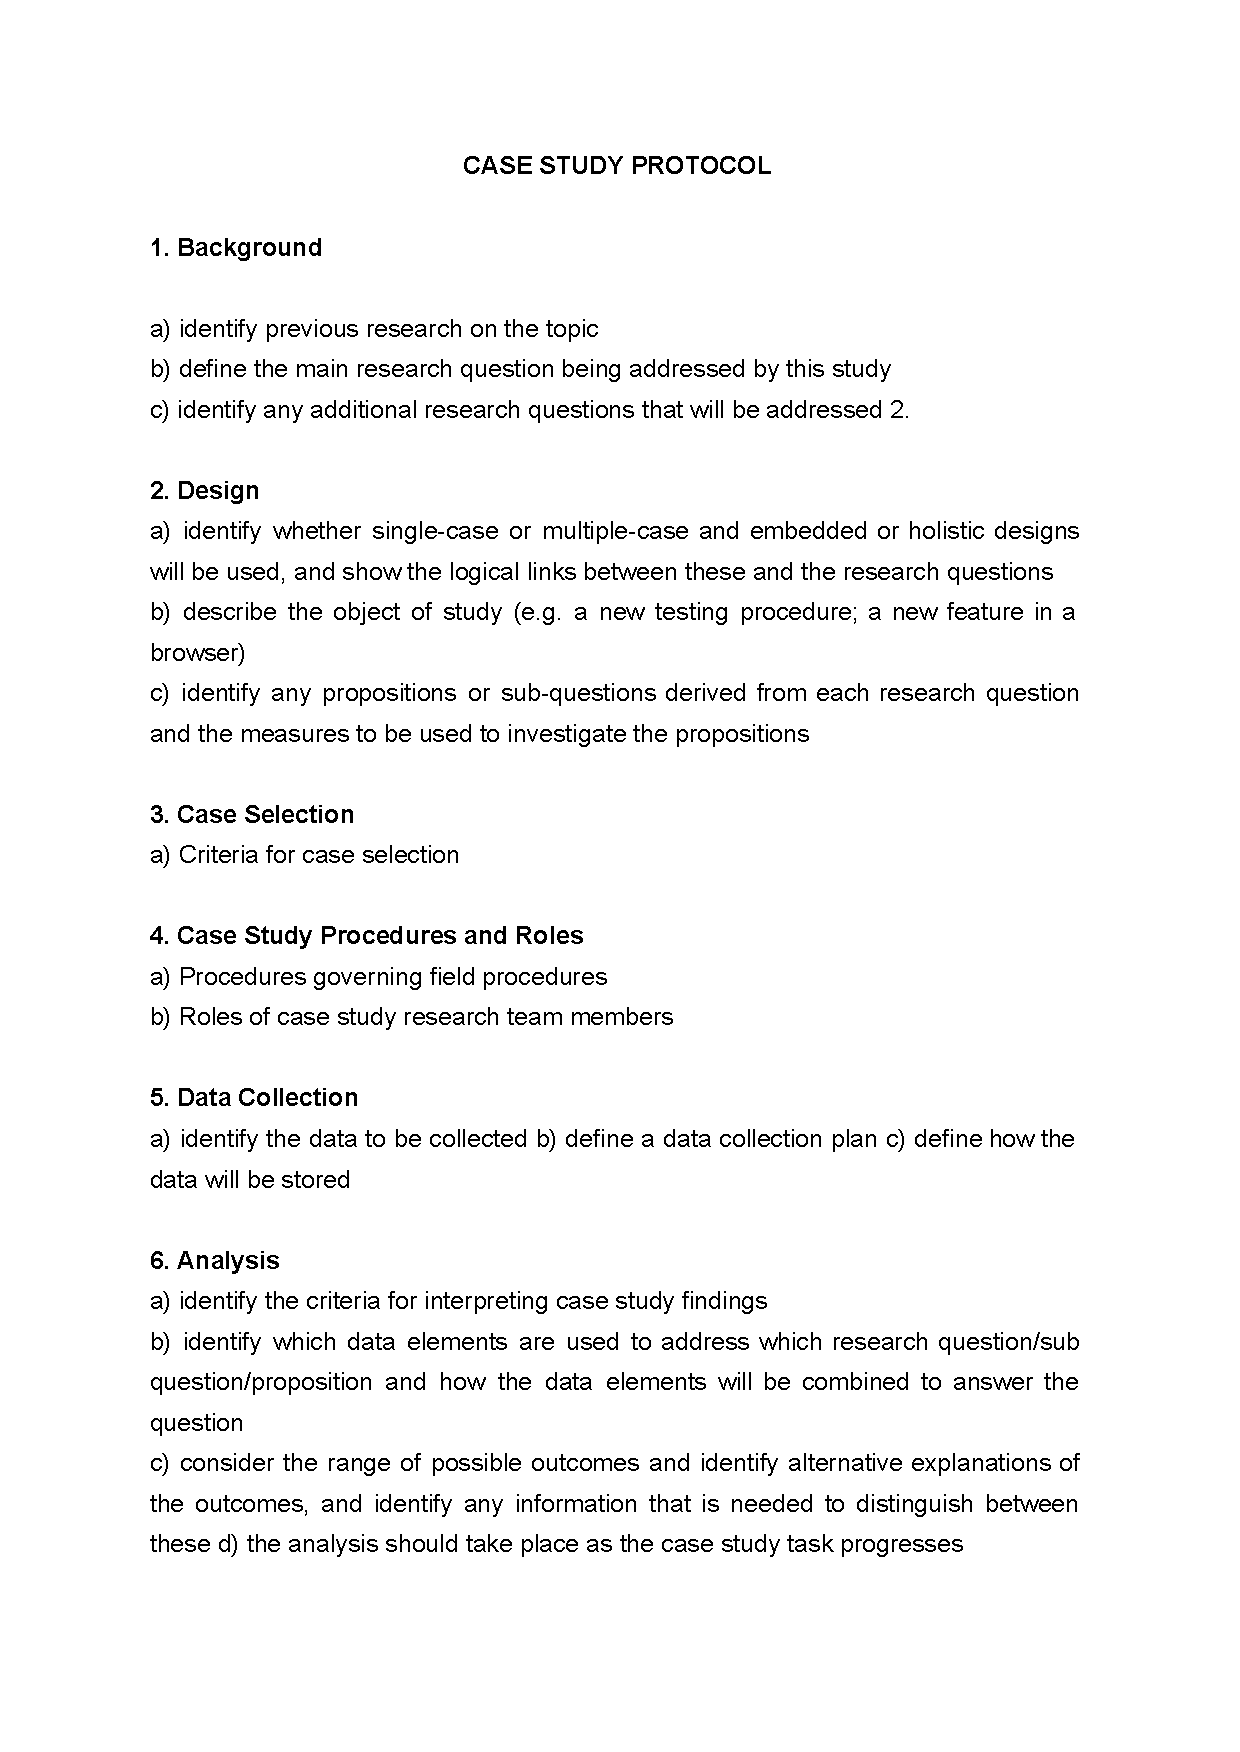
\includepdf[pages=-]{ProtocoloEstudoCaso.pdf}	

\end{anexosenv}

